\documentclass[tikz,border=5pt]{standalone}
\usepackage{pgfplots}
\pgfplotsset{compat=1.18}
\usepackage{amsmath}

\begin{document}
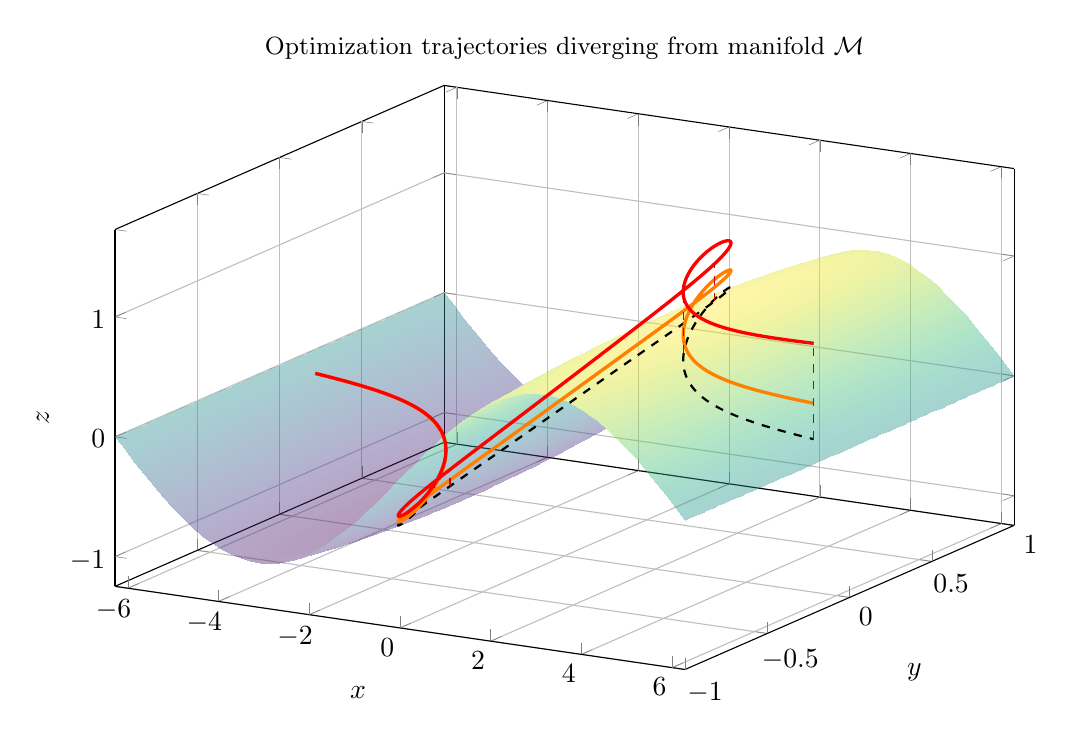
\begin{tikzpicture}
\begin{axis}[
  width=13cm,
  height=9cm,
  view={30}{25},
  xlabel={$x$},
  ylabel={$y$},
  zlabel={$z$},
  domain=-6.283:6.283,
  samples=60,
  y domain=-1:1,
  grid=major,
  colormap/viridis,
  title={Optimization trajectories diverging from manifold $\mathcal{M}$},
  title style={font=\small},
]

% --- True 2D manifold surface
\addplot3 [surf, opacity=0.4, shader=interp, draw=none]
  {sin(deg(0.5*x))*cos(deg(0.5*y))};

% Distance parameters
\pgfmathsetmacro{\omegaHigh}{0.0}
\pgfmathsetmacro{\omegaMid}{0.3}
\pgfmathsetmacro{\omegaLow}{0.8}

% --- Common starting point
\pgfmathsetmacro{\xstart}{-6.0}

% === omega_high trajectory (on manifold)
\addplot3 [
  domain=\xstart:6.0,
  samples=200,
  samples y=0,
  thick,
  dashed,
  color=black
]
({x},
 {0.5*sin(deg(x))},
 {sin(deg(0.5*x))*cos(deg(0.25*sin(deg(x))))});

% === omega_mid trajectory (quadratic divergence)
\addplot3 [
  domain=\xstart:6.0,
  samples=200,
  samples y=0,
  very thick,
  color=orange
]
({x},
 {0.5*sin(deg(x))},
 {sin(deg(0.5*x))*cos(deg(0.25*sin(deg(x)))) + \omegaMid * ((x-\xstart)/(12.0))^2});

% === omega_low trajectory (stronger quadratic divergence)
\addplot3 [
  domain=\xstart:6.0,
  samples=200,
  samples y=0,
  very thick,
  color=red
]
({x},
 {0.5*sin(deg(x))},
 {sin(deg(0.5*x))*cos(deg(0.25*sin(deg(x)))) + \omegaLow * ((x-\xstart)/(12.0))^2});

% --- Vertical connectors at selected x locations
\foreach \xx in {-6.0,-3.5,-1.0,1.5,4.0,6.0}{
  \pgfmathsetmacro{\yy}{0.5*sin(deg(\xx))}
  \pgfmathsetmacro{\zz}{sin(deg(0.5*\xx))*cos(deg(0.25*sin(deg(\xx))))}
  \pgfmathsetmacro{\zmid}{\zz + \omegaMid * ((\xx-\xstart)/(12.0))^2}
  \pgfmathsetmacro{\zlow}{\zz + \omegaLow * ((\xx-\xstart)/(12.0))^2}
  \addplot3 [orange!80!black, dashed, thin]
    coordinates {(\xx,\yy,\zz) (\xx,\yy,\zmid)};
  \addplot3 [red!80!black, dashed, thin]
    coordinates {(\xx,\yy,\zz) (\xx,\yy,\zlow)};
}

\end{axis}
\end{tikzpicture}
\end{document}

